%! Author = zhenxiang
%! Date = 23-3-24

\PassOptionsToPackage{quiet}{xeCJK}  % 抑制无意义的警告
% Preamble
\documentclass[11pt]{ctexart}

% Packages
\usepackage{amsmath}
% graphicx 插入图片
\usepackage{graphicx}
% 页面设置
\usepackage{geometry}
\geometry{left=2.5cm, right=2.5cm, top=2.5cm, bottom=2.5cm}
% codes
\usepackage{ listings}
\usepackage{xcolor}
\usepackage{color}
\definecolor{mygreen}{rgb}{0,0.6,0}
\definecolor{mygray}{rgb}{0.5,0.5,0.5}
\definecolor{mymauve}{rgb}{0.58,0,0.82}
\lstset{ %
  backgroundcolor=\color{white},   % choose the background color; you must add \usepackage{color} or \usepackage{xcolor}
  basicstyle=\ttfamily,            % the size of the fonts that are used for the code
  breakatwhitespace=false,         % sets if automatic breaks should only happen at whitespace
  breaklines=true,                 % sets automatic line breaking
  captionpos=b,                    % sets the caption-position to bottom
  commentstyle=\ttfamily\color{mygreen},    
                                   % comment style
  deletekeywords={},               % if you want to delete keywords from the given language
  escapeinside={},                 % if you want to add LaTeX within your code
  extendedchars=true,              % lets you use non-ASCII characters; for 8-bits encodings only, does not work with UTF-8
  frame=single,                    % adds a frame around the code
  keepspaces=true,                 % keeps spaces in text, useful for keeping indentation of code (possibly needs columns=flexible)
  keywordstyle=\color{blue},       % keyword style
  language=C++,                    % the language of the code
  morekeywords={},                 % if you want to add more keywords to the set
  numbers=left,                    % where to put the line-numbers; possible values are (none, left, right)
  numbersep=5pt,                   % how far the line-numbers are from the code
  numberstyle=\tiny\color{mygray}, % the style that is used for the line-numbers
  rulecolor=\color{black},         % if not set, the frame-color may be changed on line-breaks within not-black text (e.g. comments (green here))
  showspaces=false,                % show spaces everywhere adding particular underscores; it overrides 'showstringspaces'
  showstringspaces=false,          % underline spaces within strings only
  showtabs=false,                  % show tabs within strings adding particular underscores
  stepnumber=1,                    % the step between two line-numbers. If it's 1, each line will be numbered
  stringstyle=\color{mymauve},     % string literal style
  tabsize=2,                       % sets default tabsize to 2 spaces
  title=\lstname                   % show the filename of files included with \lstinputlisting; also try caption instead of title
}

% Document
\begin{document}
	
%创建目录
\tableofcontents

% CUDA PG Programming Mode
\section{Cuda-C-Programming-Guide Programming Mode Reading}


\newpage
\section{Chatgpt answer}

在CUDA中,线程块(Thread Block)、线程格(Grid of Thread Blocks)和线程(Thread)是三个不同的概念,它们的关系如下:

线程格是多个线程块的集合,通常由一个或多个线程块组成。线程格的数量可以通过$<<<...>>>$语法来指定。

线程块是多个线程的集合,由并发执行的线程组成,通常由32或64个线程组成。每个线程块都有自己的共享内存空间,并且线程块内的线程可以通过共享内存和同步操作来进行通信和协调。线程块的数量可以通过$<<<...>>>$语法中的第一个参数来指定。

线程是执行计算的最小单位,每个线程块中的所有线程都在执行同一个内核函数。每个线程都有自己的线程ID,可以通过内置变量threadIdx来访问。线程块中的所有线程共享同一个内存空间,并且可以通过共享内存和同步操作来进行通信和协调。线程的数量通常由线程块的大小($<<<...>>>$语法中的第二个参数)来指定。

线程格和线程块的关系是:线程格由多个线程块组成,每个线程块中有多个线程。线程块和线程的关系是:每个线程块由多个线程组成,每个线程有自己的线程ID。
\begin{lstlisting}
<<<numBlocks, blockSize, sharedMemSize>>>


__global__ void myKernel() {
    // kernel code here
}

int main() {
    myKernel<<<1, 64>>>();
    return 0;
}

\end{lstlisting}

总之,在CUDA中,线程格、线程块和线程都是为了实现并行计算而设计的,并且它们的组合方式可以用来实现不同类型的并行计算需求。线程格用于控制并行计算的整体规模,线程块用于控制并行计算的粒度,线程用于执行具体的计算操作。\\


当涉及到CUDA模型的内存层次和线程层次时,主要是讨论CUDA内核如何访问和操作内存以及如何在GPU上并行执行代码。

内存层次:
在CUDA中,有多个层次的内存,包括全局内存、共享内存、常量内存和纹理内存等。其中,全局内存是在设备上的全局地址空间中分配的内存,可由所有线程访问。共享内存是在线程块内的共享地址空间中分配的内存,只能被同一块内的线程访问。常量内存是只读内存,通常用于存储不变的数据,如图像数据和预计算的常量。纹理内存是一种特殊的只读内存,通常用于对图像和几何数据进行高效的访问和处理。CUDA模型提供了各种内存类型,以便GPU上的内核能够最大限度地利用内存层次结构的优势。

线程层次:
CUDA内核在GPU上并行执行,利用的是多个线程执行同一个内核函数的方式。线程的执行是分层的,由线程格、块和线程三个层次组成。线程格是最大的并行执行单位,是多个块的集合。块是线程格内的并行执行单位,是多个线程的集合。线程是最小的执行单位,是在块内的单个线程执行单个指令。CUDA模型中的线程块通常包含多个线程,这些线程可以共享共享内存、同步等资源。CUDA模型支持大规模的并行计算,可以同时执行数千个线程格和数百万个线程。\\


在CUDA中,每个线程都有一个唯一的线程ID,用于标识它在线程块中的位置。线程ID可以通过内置变量threadIdx来访问,这个变量是一个三维的向量类型(threadIdx.x、threadIdx.y和threadIdx.z),表示线程在每个维度上的索引。

例如,对于一个包含8个线程的线程块(blockSize = 8),可以使用以下方式计算每个线程的线程ID:

\begin{lstlisting}
__global__ void myKernel() {
    int tid = threadIdx.x; // 获取线程在x维度上的索引
    // 其他操作...
}
//包含4个维度的线程块和线程格
dim3 blockSize(16, 16, 8, 2);
dim3 gridSize(8, 8, 4, 1);
myKernel<<<gridSize, blockSize>>>();

\end{lstlisting}

为什么threadIdx, blockIdx, blockDim定位线程用xyz,而不用下角标123?

使用x、y、z来定位线程的原因是因为CUDA C中的线程块和线程网格是一个三维的结构,每个维度都有对应的坐标。因此,使用x、y、z作为索引可以很方便地对应到每个维度。如果使用下角标123,则需要额外说明这些数字对应于哪个维度,更容易混淆和出错。同时,x、y、z也更符合空间坐标系的表示方法,更容易理解。

PTX是一种中间表示语言,用于将CUDA程序源代码转换为适用于不同GPU架构的机器代码。PTX代码可以被JIT(Just-In-Time)编译器或静态编译器编译为适用于特定GPU架构的机器代码。由于PTX是一种中间表示语言,因此它可以跨不同的GPU架构进行优化和转换,从而提高程序的可移植性和性能。

\newpage
\section{Data parallel computing}
Programing Massively Parallel Processors :  Chapter 2.

许多代码示例将用于说明编写可扩展并行程序的关键概念。为此,我们需要一种简单的语言,支持大规模并行和异构计算,我们选择使用CUDA C作为我们的代码示例和练习。CUDA C扩展了流行的C编程语言,具有最小的新语法和接口,以便程序员可以针对同时包含CPU核心和大规模并行GPU的异构计算系统。正如名称所示,CUDA C是建立在NVIDIA的CUDA平台上的。CUDA目前是最成熟的大规模并行计算框架。它在高性能计算行业广泛使用,并提供了复杂的工具,如编译器、调试器和分析器,可在最常见的操作系统上使用。

一个重要的点:虽然我们的示例大多使用CUDA C,因为它简单易用且广泛使用,但CUDA平台支持许多语言和应用程序编程接口(API),包括C ++、Python、Fortran、OpenCL、OpenACC、OpenMP等。CUDA实际上是一种支持一组概念来组织和表达大规模并行计算的体系结构。我们教授的正是这些概念。为了让其他语言(C++、FORTRAN、Python、OpenCL等)的开发人员受益,我们提供附录展示如何将这些概念应用于这些语言。\\
% \par\noindent 命令用于在新行中开始一段文本,并清除缩进。\hrulefill 命令创建一条可拉伸的横线,并在行的末尾填充空间。最后,\par 命令用于在横线下方开始一个新行。
\par\noindent\hrulefill\par % /单独一行起一道横线
% 如果您希望横线具有特定的宽度或高度,可以使用 \rule 命令。例如,要创建一个宽度为 5 厘米、高度为 0.5 毫米的横线,可以使用以下代码:
% \par\noindent\rule{17cm}{0.5mm}\par

\subsection{Data Parallelism }

当现代软件应用程序运行缓慢时,问题通常是要处理太多数据。消费者应用程序操作图像或视频,其中包含数百万到数万亿个像素。科学应用程序使用数十亿的网格单元来模拟流体动力学。分子动力学应用程序必须模拟数千到数百万个原子之间的相互作用。航空公司排班涉及到数千个航班、机组人员和机场登机口。重要的是,这些像素、粒子、单元、相互作用、航班等大部分都可以独立处理。将彩色像素转换为灰度只需要该像素的数据。模糊图像通过将每个像素的颜色与附近像素的颜色取平均值,只需要该小邻域像素的数据。甚至看似全局的操作,如查找图像中所有像素的平均亮度,也可以分解成许多可以独立执行的小型计算。这种独立的计算形式是数据并行性的基础:将计算围绕数据(重新)组织,使我们可以并行执行独立的计算以更快地完成整个任务,通常比顺序执行快得多。

\subsubsection{TASK PARALLELISM VS. DATA PARALLELISM}

数据并行不是并行编程中唯一使用的并行方式。任务并行同样在并行编程中得到广泛应用。任务并行通常通过任务分解来实现应用程序。例如,一个简单的应用程序可能需要执行矢量加法和矩阵-向量乘法,每个操作都是一个任务。如果这些任务可以相互独立地执行,那么就存在任务并行。I/O和数据传输也是任务的常见来源。

在大型应用程序中,通常存在更多的独立任务,因此也存在更多的任务并行性。例如,在分子动力学模拟器中,自然任务列表包括振动力、旋转力、非键作用的邻居识别、非键作用、速度和位置以及基于速度和位置的其他物理属性。

总的来说,数据并行是实现并行程序可扩展性的主要来源。对于大型数据集,人们通常可以找到丰富的数据并行性,以便利用大规模并行处理器,并允许应用程序性能随着每一代具有更多执行资源的硬件而增长。然而,任务并行也可以在实现性能目标方面发挥重要作用。我们将在介绍流时介绍任务并行。

数据并行和任务并行是并行计算中两种常用的并行模式,它们之间存在一些区别和联系。

\textbf{区别}:

数据并行:将相同的操作应用于不同的数据集合,每个操作都是独立的,可以同时进行,例如在一组图像上应用滤波器。
任务并行:将不同的操作分配给不同的处理器核心或线程,每个操作相互依赖,需要按照特定的顺序执行,例如在一个模拟器中计算不同的物理效应。

\textbf{联系}:


数据并行和任务并行都可以提高程序的并行度,从而加速程序的执行。
在实际的并行应用中,常常需要同时使用数据并行和任务并行,例如在一个大规模的科学模拟程序中,可以通过将不同的模拟任务分配给不同的处理器核心,并对每个模拟任务使用数据并行技术来提高整个程序的性能。
总之,数据并行和任务并行是并行计算中两种常用的并行模式,它们可以分别或者同时应用于不同的并行应用中,以提高程序的并行性和性能。
% 图片置于当前位置
\begin{figure}[ht]
	\centering
	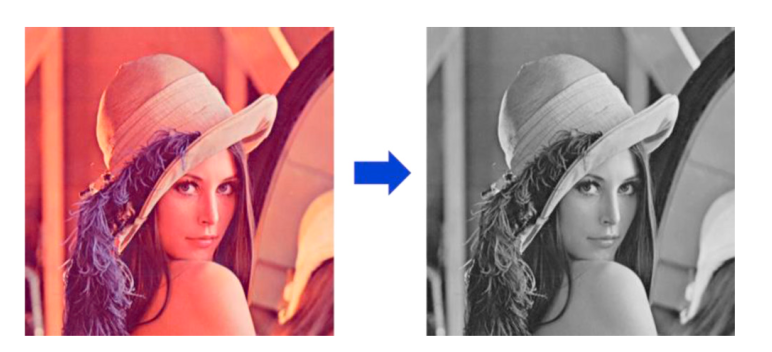
\includegraphics[width=0.8\textwidth]{photos/colorimage.png}
	\caption{Conversion of a color image to a greyscale image}
	\label{fig:1}
\end{figure}
我们将在接下来的章节中使用图像处理作为运行示例的来源。让我们通过上面提到的颜色转灰度示例来说明数据并行的概念。图2.1显示了一个彩色图像(左侧),由许多像素组成,每个像素包含从0(黑色)到1(完全强度)变化的红色、绿色和蓝色分数值(r、g、b)。

\subsubsection{RGB COLOR IMAGE REPRESENTATION}

在RGB表示法中,图像中的每个像素都被存储为一个(r, g, b)值的元组。一行图像的格式是(r g b)(r g b)...(r g b),如下面的概念图所示。每个元组指定了红色(R)、绿色(G)和蓝色(B)的混合比例。也就是说,对于每个像素,r、g和b值表示在呈现该像素时,红色、绿色和蓝色光源的强度(0为暗,1为全强度)。

在实际应用中,允许的这三种颜色的混合比例因行业而异。这里,以AdobeRGB颜色空间中的有效混合比例为例,其混合比例呈三角形内部。每种混合比例的垂直坐标(y值)和水平坐标(x值)表示应该赋予G和R的像素强度分数。剩余的像素强度分数(1-y-x)应该分配给B。为了渲染图像,每个像素的r、g、b值被用来计算像素的总强度(亮度)以及混合系数(x,y,1-y-x)。

% 图片置于当前位置
\begin{figure}[ht]
	\centering
	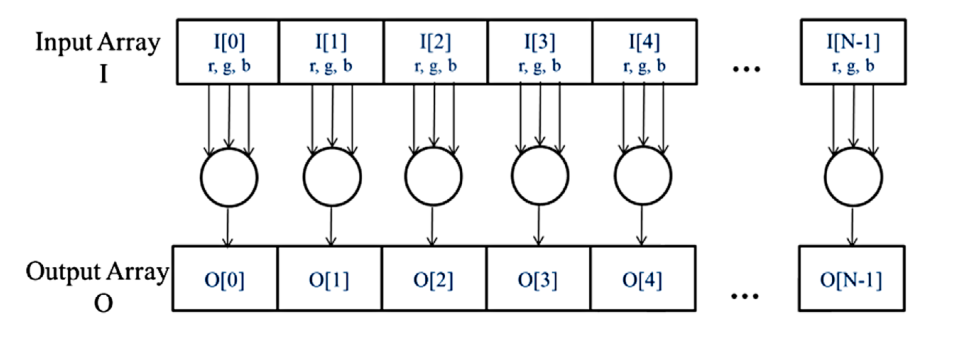
\includegraphics[width=0.8\textwidth]{photos/pixels.png}
	\caption{The pixels can be calculated independently of each other during color to greyscale
		conversion.}
	\label{fig:2}
\end{figure}

将彩色图像(图2.1左侧)转换为灰度图像(右侧),我们通过应用以下加权求和公式来计算每个像素的亮度值L:

\begin{equation}
	L= r*0.21 + g * 0.72 + b *0.07
\end{equation}

如果我们将输入视为一个以 RGB 值组织的图像数组 I,输出为相应的亮度值数组 O,我们可以得到如图2.2所示的简单计算结构。例如,O [0] 是通过根据上述公式计算 I [0] 中的 RGB 值的加权和来生成的;O [1] 是通过计算 I [1] 中的 RGB 值的加权和生成的,O [2] 是通过计算 I [2] 中的 RGB 值的加权和生成的,以此类推。这些像素级计算中的任何一个都不依赖于其他计算;所有计算都可以独立执行。显然,颜色到灰度的转换展现了丰富的数据并行性。当然,完整应用程序中的数据并行性可能更为复杂,本书的大部分内容都致力于教授发现和利用数据并行性所需的“并行思维”。

\subsection{A VECTOR ADDITION KERNE}

A simple traditional vector addition C code example.


\begin{lstlisting}
#include <cuda.h>
…
void vecAdd(float* A, float* B, float* C, int n)
{
	int size = n* sizeof(float);
	float *d_A *d_B, *d_C;
	…
	1. // Allocate device memory for A, B, and C
	// copy A and B to device memory
	2. // Kernel launch code – to have the device
	// to perform the actual vector addition
	3. // copy C from the device memory
	// Free device vectors
}	
\end{lstlisting}


\subsection{Device global memory and data transfer}

We now use a simple code example to illustrate the use of cudaMalloc.

\begin{lstlisting}
float *d_A;
int size=n * sizeof(float);
cudaMalloc((void**)&d_A, size);
...
cudaFree(d_A);
	
\end{lstlisting}

为了清晰起见,我们将一个指针变量以字母“d\_”开头,表示它指向设备内存中的一个对象。程序将指针d\_A的地址(即\&d\_A)作为void指针进行转换后,作为第一个参数传递。也就是说,d\_A将指向为A向量分配的设备内存区域。分配区域的大小将是n个单精度浮点数的大小,这在今天的大多数计算机上是4个字节。在计算完成后,使用指针d\_A作为输入调用cudaFree以释放A向量的存储空间,从设备全局内存中释放它。请注意,cudaFree不需要更改指针变量d\_A的内容;它只需要使用d\_A的值将已分配的内存重新输入可用池中。因此,只传递值,而不是d\_A的地址作为参数。

\textbf{指针d\_A的变化:}

在调用 cudaMalloc 函数之前,指针 d\_A 是未初始化的,也就是不指向任何一个内存地址。因此,在使用 d\_A 之前需要先为它分配内存,否则访问该指针可能会导致未定义的行为。在 cudaMalloc 函数被调用之后,d\_A 将会指向分配给 A 向量的设备内存地址。在 cudaFree 函数被调用之后,d\_A 将会变成未初始化的状态,也就是不再指向任何有效的内存地址。

cudaMemcpy函数有四个参数。第一个参数是指向要复制的数据对象目标位置的指针。第二个参数指向源位置。第三个参数指定要复制的字节数。第四个参数指示复制涉及的内存类型:从主机内存到主机内存,从主机内存到设备内存,从设备内存到主机内存和从设备内存到设备内存。例如,内存复制函数可以用于将数据从设备内存的一个位置复制到设备内存的另一个位置。\\

cudaMemcpy()

\begin{itemize}
	\item Memory data transfer
	\item Requires four parameters
	\begin{itemize}
		\item[$\circ$] Pointer to destination
		\item[$\circ$] Pointer to source
		\item[$\circ$] Number of bytes copied
		\item [$\circ$] Type/Direction of transfer
		\end{itemize}
\end{itemize}

\begin{lstlisting}
cudaMemcpy(d_A, A, size, cudaMemcpyHostToDevice);
cudaMemcpy(d_B, B, size, cudaMemcpyHostToDevice);
cudaMemcpy(C, d_C, size, cudaMemcpyDeviceToHost);
\end{lstlisting}



请注意,目前cudaMemcpy不能在多GPU系统中用于在不同GPU之间复制数据。

We show a more complete version of the vecAdd function.

\begin{lstlisting}
void vecAdd(float* h_A, float* h_B, float* h_c, int n){
	int size = n * sizeof(float);
	float *d_A, *d_B, *d_C;
	
	cudaMalloc ((void **)   &d_A,    size);
	cudaMemcpy(d_A, h_A, size, cudaMemcpyHostToDevice);
	cudaMalloc ((void **)   &d_B,    size);
	cudaMallocpy(d_B, h_B, size, cudaMemcpyHostToDevice);
	
	cudaMalloc((void **)   &d_C,  size);
	
	// Kernel invocation code - to be shown later
	...
	
	cudaMallocpy(d_B, h_B, size, cudaMemcpyHostToDevice);
	// Free device memory for A, B, C
	cudaFree(d_A); cudaFree(d_B); cudaFree(d_C);
} 
\end{lstlisting}

代码错误检查

\begin{lstlisting}
cudaError_t err=cudaMalloc((void **) &d_A, size);
if (error !=cudaSuccess) {
	printf(“%s in %s at line %d\n”, cudaGetErrorString(err),__
	FILE__,__LINE__);
	exit(EXIT_FAILURE);
}
\end{lstlisting}


\subsection{KERNEL FUNCTIONS AND THREADING}


\begin{lstlisting}
// Compute vector sum C = A+B
// Each thread performs one pair-wise addition
__global__
void vecAddKernel(float* A, float* B, float* C, int n)
{
	int i = blockDim.x*blockIdx.x + threadIdx.x;
	if(i<n) C[i] = A[i] + B[i];
}
\end{lstlisting}




\begin{lstlisting}
int vectAdd(float* A, float* B, float* C, int n)
{
	// d_A, d_B, d_C allocations and copies omitted
	// Run ceil(n/256) blocks of 256 threads each
	vecAddKernel<<<ceil(n/256.0), 256>>>(d_A, d_B, d_C, n);
}
\end{lstlisting}

解释一下为什么用ceil:

在CUDA中,每个线程块的大小通常是固定的,因为它们是在GPU的多处理器上执行的。在这个例子中,每个线程块的大小被设置为256个线程。

但是,当需要处理的向量长度不是256的整数倍时,就需要计算需要多少个线程块来处理所有的数据。为了确保处理所有的数据,需要向上取整到最近的整数块数。

因此,ceil(n/256.0)被用来计算所需的线程块数,并向上取整以确保所有的数据都被处理。

\subsection{KERNEL LAUNCH}

A complete version of the host code in the vecAdd.function.

\begin{lstlisting}
	void vecAdd(float* h_A, float* h_B, float* h_c, int n){
		int size = n * sizeof(float);
		float *d_A, *d_B, *d_C;
		
		cudaMalloc ((void **)   &d_A,    size);
		cudaMemcpy(d_A, h_A, size, cudaMemcpyHostToDevice);
		cudaMalloc ((void **)   &d_B,    size);
		cudaMallocpy(d_B, h_B, size, cudaMemcpyHostToDevice);
		
		cudaMalloc((void **)   &d_C,  size);
		
		vecAddKernel<<<ceil(n/256.0), 256>>>(d_A, d_B, d_C, n);
		
		cudaMallocpy(d_B, h_B, size, cudaMemcpyHostToDevice);
		// Free device memory for A, B, C
		cudaFree(d_A); cudaFree(d_B); cudaFree(d_C);
	} 

// Compute vector sum C = A+B
// Each thread performs one pair-wise addition
__global__
void vecAddKernel(float* A, float* B, float* C, int n)
{
	int i = blockDim.x*blockIdx.x + threadIdx.x;
	if(i<n) C[i] = A[i] + B[i];
}

\end{lstlisting}

\subsection{SUMMARY}

本章提供了CUDA C编程模型的快速简化概述。CUDA C扩展了C语言以支持并行计算。我们在本章讨论了其中一个基本子集。为了方便起见,我们将在下面总结我们在本章中讨论过的扩展:
\begin{itemize}
	\item \_global\_函数:在设备上执行的函数,由主机调用。
	\item threadIdx, blockIdx, blockDim:内置的线程索引和块索引变量,可用于访问线程和块的ID。
	\item $<<<gridDim, blockDim>>>$:用于指定要在设备上执行的内核函数的线程块和线程数。
	\item cudaMalloc和cudaFree:用于在设备上分配和释放内存。
	\item cudaMemcpy:用于在主机和设备之间复制内存。
	\item 向量加法示例:展示了如何使用CUDA C实现简单的并行计算。
\end{itemize}


\end{document}